\section{Evaluation}
\label{sec:evaluation}
\subsection{Experimental Setup}
\subsubsection{\textbf{Model Mining}}
\begin{figure}
	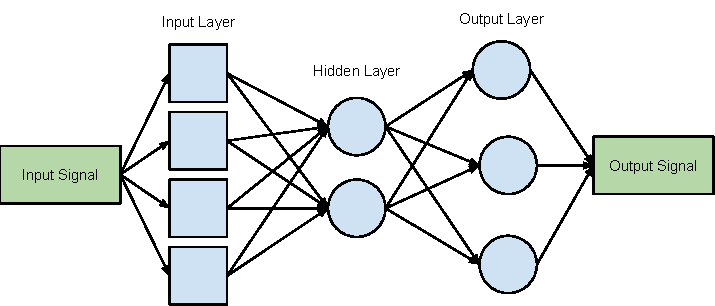
\includegraphics[width=0.8\linewidth]{mlp}
	\centering
	\caption{MLP Structure}
	\label{fig:mlp}
	%\vspace{15pt}
\end{figure}
We have mined {\bf x} multilayer perceptron (MLP) models from 3000 Keras repositories. However, there are many different kinds of machine learning models in 3000 Keras repositories. Thus, we have to identify which model is MLP. To address this problem, we need to identify the general structure of MLP. Then, we filter the models which are not belong to this structure. Figure \ref{fig:mlp} represent a general structure of MLP. There are three components in MLP's structure which are input layer, hidden layer, output layer. Moreover, all of these layer are constructed by using Dense layer and activation layer. Therefore, if a mined model have another kinds of layer like convolutional layer or recurrent layer, it will be discarded. To detect and extract MLPs, we have used control flow graph (CFG). In particular, we manually collect a list of the Keras APIs used to build Keras models. Then, the CFG parses through each statement of the Python files and collect the API names. If the API names is belong to the APIs list, we will collect them. After that, we connect all the API calls together to acquire a complete model. If a model contains at least one API which are not used for constructing MLP, we will remove it. Moreover, we also filter the MLP models which miss some requirement information like input shape or output channel.
\begin{figure}
	\centering
	\begin{subfigure}[b]{.45\linewidth}
		\begin{lstlisting}[basicstyle=\tiny,numberblanklines=false]
		model.add(Dense(units=64, activation='relu', input_dim=100)) 
		
		model.add(Dense(units=10, activation='softmax'))
		\end{lstlisting}
		\caption{Original MLP}
		\label{fig:originalCNN}
	\end{subfigure}
	\begin{subfigure}[b]{.45\linewidth}
		\begin{lstlisting}[basicstyle=\tiny,numberblanklines=false]	
		{'func': 'Dense', 'input_dim':100, 'units': 64} 
		{'func': 'relu'}
		{'func': 'Dense', 'units': 64}
		{'func': 'softmax'}
		\end{lstlisting}
		\caption{ANN}
		\label{fig:convertedCNN}
	\end{subfigure}
	\caption{Original MLP vs ANN}
	\label{fig:converted}
\end{figure}



To be easier in using the mined models, we have stored them in form of abstract neural network (ANN). Figure \ref{fig:converted} shows the example of original MLP and ANN. ANN is a graph whose nodes represent for model layers and edges represent for the order of the layers. For example, the first line is Dense layer which includes three information which are 100 input channel, 64 output channel, and Relu activation. Actually, Relu activation is a layer; thus, we seperate this layer in two layer, Dense layer and activation layer.
\begin{algorithm}
	\caption{Model Mining}\label{euclid}
	\begin{algorithmic}[1]
		\Procedure{model\_extraction}{pyFiles}
			\State $\textit{CFG} \gets \text{py}$
			\State \Return MLP
		\EndProcedure
		\Procedure{model\_filtering}{pyFiles}
		\State $\textit{check = True} $
		\For{$py$ $\in$ $pyFiles$}
			\State $\textit{check = True} $
			\State $model$ = $model\_extraction(py)$ 
			\For{$layer$ $\in$ $model$}
				\If {$layer$ $is$ $False$} 
					\State $\textit{check = False} $
					\State {\bf break}
				\EndIf
			\EndFor
			\If {$check$ $=$ $True$} 
				\State $\textit{ANN}  \gets \text{model}$
			\EndIf
		\EndFor
		
		\EndProcedure	
	\end{algorithmic}
\end{algorithm}


\subsubsection{Evaluation Metrics}

\subsection{Experimental Methodology}
RQ1: What is the best value for $\delta$.
Using model mining, we will emprically evaluate the $\delta$ value.

RQ2: How efficient is this approach?

RQ3: How effective is this approach?


%\subsection{Results}




%\subsection{Analysis}




%\subsection{Summary}




